
%title page
\begin{frame}
\titlepage
\end{frame}

\section{High-energy \texorpdfstring{$\gamma$}{gamma} sources}

\begin{frame}{Why to study?}
  \begin{itemize}
    \item $\gamma$-rays:
    \begin{itemize}
	\item are not deflected by interstellar magnetic fields $\Rightarrow$ can be tracked to their origin;
	\item can be used for point sources search;
	\item are able to provide answers about the Galactic cosmic ray propagation;
	\item $\gamma$-ray flux study could bring us insights on cosmic rays acceleration mechanisms.
    \end{itemize}
    \item high-energy $\gamma$ (above 100~TeV):
    \begin{itemize}
	\item not so well-investigated because of flux intensity decrease for all CR particles at higher energies;
	\item are supposed to be produced by black holes, neutron stars, supernova remnants, super-bubbles / star-forming regions / young massive star clusters;
	\item could improve our understanding about properties of matter in extreme states that cannot be studied in laboratories.
    \end{itemize}
  \end{itemize}
\end{frame}

\begin{frame}{HAWC high-energetic $\gamma$-ray sources}

\begin{itemize}
  \item six sources in the Galactic plane that emit above 56~TeV:
\end{itemize}
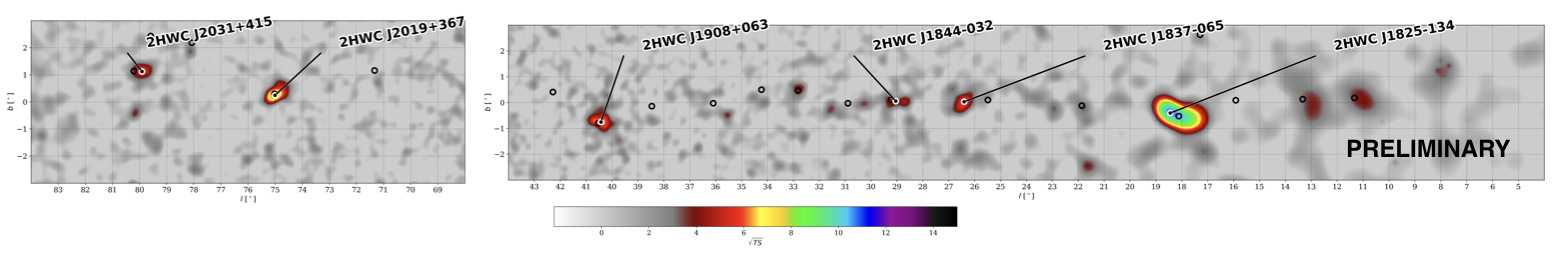
\includegraphics[width=1\textwidth]{pics/HWC_above_56TeV.png}
\begin{itemize}
  \item two of them continue to emit past 100~TeV:
\end{itemize}
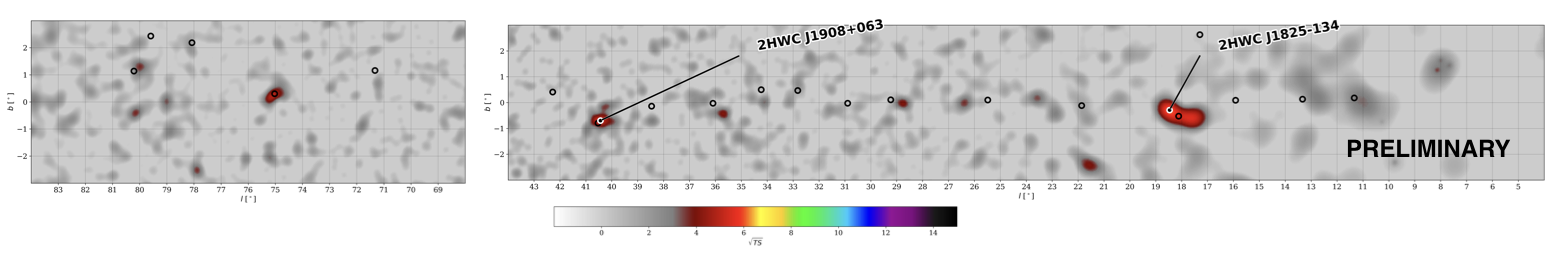
\includegraphics[width=1\textwidth]{pics/HWC_above_100TeV.png}

Malone, K. (2018). A survey of the highest-energy astrophysical sources with the HAWC Observatory (Doctoral dissertation).
Retrieved from https://hawc-observatory.org/publications/docs/Malone-Dissertation.pdf

\end{frame}

\begin{frame}{Carpet-2 extensive air shower array}
\begin{itemize}
 \item located at the Baksan Neutrino Observatory of INR RAS;
\end{itemize}
\vspace{-0.3em}
\begin{minipage}[c]{0.5\textwidth}
\begin{itemize}
 \item consists of:
 \begin{itemize}
  \item surface array to detect the electromagnetic CR components;
  \item underground scintillator detectors to detect the muonic component;
 \end{itemize}
\item used for study air showers induced by particles with primary energy above 50 TeV.
\item the main area $\approx 200$~m$^2$.
\end{itemize}
\end{minipage}
\hfill
\begin{minipage}[c]{0.49\textwidth}
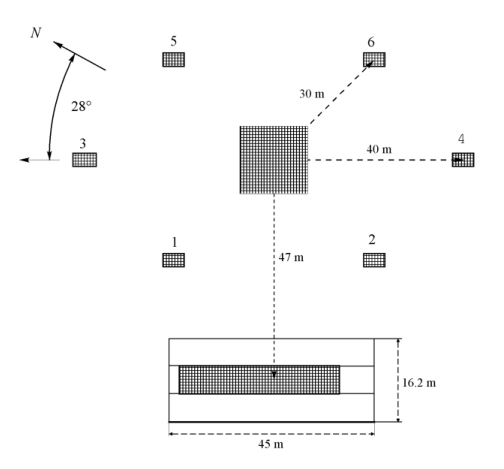
\includegraphics[width=1\textwidth]{pics/CarpetLayout.pdf}
\end{minipage}
% TODO: add picture of the layout on this slide!
\end{frame}

\begin{frame}{Carpet-2 high-energy gamma rays search for IceCube point sources}
% - применили multi-messndger approach: наблюдали за потоком гамма со стороны IceCube high-energy (appr. 100 Tev) neutrino sources;
% (рисунок фейнмановской диаграммы?)
\begin{itemize}
  \item 34 published IceCube high-energy neutrino events;
%  \item arrival directions, while 13.6 are expected
% from isotropy. This resulted in the published 
  \item 95\% CL upper limit on total steady flux of $E_{\gamma} > 1$~PeV photons: $8.5 \times 10^{-15}$~cm$^{-2}$s$^{-1}$. 
  \item 95\% CL upper limit on fluence of $E_{\gamma} > 1$~PeV photons for the IceCube EHE3 flare: $4.4 \times 10^{-5}$~PeV/cm$^2$.
\end{itemize}
\small
\begin{itemize}
  \item[{[1]}] D.D.~Dzhappuev et al., \textit{Carpet-2 search for PeV gamma rays associated with IceCube high-energy neutrino events}, arXiv:1812.02662 [astro-ph.HE].
  \item[{[2]}] D.D.~Dzhappuev et al., \textit{Search for astrophysical PeV gamma rays from point sources with Carpet-2}, arXiv:1812.02663 [astro-ph.HE].
\end{itemize}

% \item Used the events recorded in the 2016: 18 runs to search for coincidences with IceCube events in direction and time.
% \item Constrain the potential flux of photons with energy $E_{\gamma} > 1$~PeV to be $< 5.4 \cdot 10^-5$~PeV/cm$^2$ with 95\% CL.
\end{frame}
